\documentclass{article}

\textwidth=6.5in
\textheight=8.5in
\voffset=-54pt
\oddsidemargin=0in
\evensidemargin=0in
\setlength{\parskip}{8pt}
\setlength{\parindent}{0pt}

\usepackage[normalem]{ulem}

\usepackage{amsmath, amssymb}
\usepackage{ifthen}

\usepackage[inline]{enumitem}
\setlist{topsep=0pt}

\usepackage{xcolor}
\usepackage[pdftex]{graphicx}

% change hyperref options
\PassOptionsToPackage{hyphens}{url}
\usepackage[bookmarks,colorlinks,linkcolor=black,citecolor=blue,pdfstartview=FitH,urlcolor=black]{hyperref}
\hypersetup{pdfpagemode=UseNone}

\usepackage{graphicx}
\usepackage{multicol}
\usepackage{framed}
\usepackage{array}
\usepackage{icomma}
\usepackage{microtype}
\usepackage{diffcoeff}[=v4]

\usepackage{soul}

\usepackage{pgfplots}
\pgfplotscreateplotcyclelist{mycolor}{%
  black, blue, red, green!70!black,magenta,
  purple, cyan, orange
}
\pgfplotsset{
  cycle list name=mycolor,
  axis lines=middle,
  every axis plot/.style={no marks, thick},
  every axis/.style={
    enlarge x limits=false,
    enlarge y limits=auto,
    xlabel style={at={(current axis.right of origin)},anchor=west},
    ylabel style={at={(current axis.above origin)},anchor=south},
    % extra x and y ticks for asymptotes
    extra x tick style={grid=major, grid style={dashed,black}},
    extra y tick style={grid=major, grid style={dashed,black}},
    /pgf/number format/1000 sep={},
  },
  tick label style = {font=\footnotesize, fill=white, inner sep=0pt},
  xticklabel shift=1pt,    
  scaled ticks=false,
  scaled y ticks=false,
  unbounded coords=jump,
  samples=101,
  minor tick length=0,
  scatter/classes={
    open={mark=*,draw=black,fill=white, mark size=2, thin},
    closed={mark=*,draw=black,fill=black, mark size=2, thin}
  },
  compat=1.18
}

\usepackage{tikz}
\usetikzlibrary{
  % enables the snake paths
  decorations.pathmorphing,%
  % enables bigger arrows
  decorations.markings,%
  decorations.pathreplacing,%
  decorations.text,%
  calc,%
  patterns,%
  shapes.geometric,%
  arrows,
  decorations.shapes,
  positioning,
  plotmarks,
}
\tikzset{>=latex} % sets default arrow type in tikz
\tikzset{font=\small}

\interfootnotelinepenalty=10000
\renewcommand{\thefootnote}{(\arabic{footnote})}

\usepackage{multirow, bigdelim}

\newcommand\iscurrentenumi[1]{%
  \ifthenelse{\equal{#1}{\theenumi}}{}{#1}}
\setenumerate[1]{ref=\#\arabic*}
\setenumerate[2]{ref=\protect\iscurrentenumi{\theenumi}(\alph*)}
\newcommand\enumiiprefix[2]{%
  \ifthenelse{{\equal{#1}{\theenumi}}\AND{\equal{#2}{(\alph{enumii})}}}{}{}%
  \ifthenelse{{\equal{#1}{\theenumi}}\AND{\NOT{\equal{#2}{(\alph{enumii})}}}}{#2}{}%
  \ifthenelse{\equal{#1}{\theenumi}}{}{#1#2}%
}
\setenumerate[3]{ref=\protect\enumiiprefix{\theenumi}{(\alph{enumii})}\roman*}

\definecolor{ideacolor}{rgb}{0.7,0,0}
\newcommand{\ideas}[1]{\color{ideacolor} #1 \color{black}}
\newcommand{\ideacolor}{maroon}

\newlength{\tipmargin}
\makeatletter
\newcommand{\version}[2]{\ifthenelse{\equal{#1}{1a}}{#2}{}}

\renewenvironment{framed}{
  \setlength{\tipmargin}{\textwidth-\linewidth}
  \advance\@totalleftmargin-\tipmargin
  \def\FrameCommand{\hspace{\tipmargin}\fbox}%
  \advance\linewidth\tipmargin
  \MakeFramed {\advance\hsize-\width \FrameRestore}%
}
{\endMakeFramed}

\def\pr@m@s{%
  \ifx'\@let@token
    \expandafter\pr@@@s
  \else
    \ifx^\@let@token
      \expandafter\expandafter\expandafter\pr@@@t
    \else
      \expandafter\expandafter\expandafter\pr@@@end
    \fi
  \fi}
\def\pr@@@end{\egroup
    \@ifnextchar({\mkern-2mu }{\@ifnextchar\{{\mkern-2mu }{\@ifnextchar[{\mkern-.5mu }{}}}}

\makeatother

\newlength{\highlightwidth}
\newcommand{\highlight}[1]{\setlength{\highlightwidth}{\linewidth}%
  \addtolength{\highlightwidth}{-55pt}%
  \hspace{24pt}\begin{minipage}[t]{\highlightwidth} \setlength{\parskip}{8pt} #1 \end{minipage}\hspace{24pt}}

\definecolor{purple}{rgb}{0.5,0,1.0}

\newcommand{\textbook}[0]{\href{http://isites.harvard.edu/fs/docs/icb.topic1511355.files/fullbook.pdf}{textbook}}

% change to \usepackage[sols]{handout} to see solutions
\usepackage[]{handout}
\renewcommand{\workshopnote}{CA Notes.}    

\begin{document}

\htitle{Worksheet 2 - The Chain Rule, Continued}
\begin{problemonly}
    \begin{framed}

You should be able to:

\begin{itemize}[topsep=0pt,partopsep=0pt,parsep=8pt,itemsep=0pt]

\item You should be able to apply the Chain Rule like a pro!

\item You should be able to apply the Chain Rule in more general contexts,
  such as in a word problem or when given a composition of functions
  described by graphs or numerical data.

\item You should understand how logarithms and the Chain Rule can be used
  to show that the Power Rule $\tfrac{d}{dx} \left( x^n \right) =
  nx^{n-1}$ holds for any real number $n$. 

\end{itemize} 

    \end{framed}
\end{problemonly}

\begin{enumerate}
\item 
{\bf Warm-up} Fill in the first table, recalling the derivatives we've learned over the last month.
\begin{center}
    \begin{tabular}{| l | l | c | l | l |}
      \multicolumn{2}{c}{Table 1: Derivatives we knew before} &
      \multicolumn{1}{c}{} 
      & \multicolumn{2}{c}{Table 2: Derivatives with the Chain Rule} \\ 
      \cline{1-2} \cline{4-5} & & & & \\
      $f(x) = x^n$ & $f'(x) = \solonly{nx^{n-1}}$ \hspace{0.4in} &
      \hspace{0.5in} &
      $h(x) = [g(x)]^n$ & $h'(x) = \solonly{n[g(x)]^{n-1}g'(x)}$
      \hspace{0.9in} \\ 
      & & & & \\
      $f(x) = e^{kx}$ & $f'(x) = \solonly{ke^{kx}}$ & & $h(x) = e^{g(x)}$
      & $h'(x) = \solonly{e^{g(x)}g'(x)}$ \\ 
      & & & & \\
      $f(x) = b^{x}$ & $f'(x) = \solonly{\ln(b)b^x}$ & & $h(x) = b^{g(x)}$
      & $h'(x) = \solonly{\ln(b)b^{g(x)}g'(x)}$ \\ 
      & & & & \\
      $f(x) = \ln x$ & $f'(x) = \solonly{\frac{1}{x}}$ & & $h(x) = \ln
      [g(x)]$ & 
      $h'(x) = \solonly{\frac{g'(x)}{g(x)}}$ \\ 
      & & & & \\
      \cline{1-2} \cline{4-5} 
    \end{tabular}
  \end{center}
  


\item 
  \note{This is meant to show students why the Power Rule works for
    non-integer exponents.  It's also good practice with logs and
    exponents.}  

  Earlier this semester, we learned the Power Rule, which said that $\frac{d}{dx} x^n
  = n x^{n-1}$ for any real number $n$.  However, we only \textit{proved}
  this when $n$ was either a positive integer or $\frac{1}{2}$.  Now that
  we know the Chain Rule, we can finally prove the Power Rule for all real
  numbers $n$.  In this problem, you'll use the Chain Rule to prove that
  the derivative of $x^{\pi}$ is $\pi x^{\pi - 1}$.  (The same idea works
  for any exponent, not just $\pi$.)

  \begin{enumerate}
  \item
    \begin{problem}[\vfill]
      Rewrite $f(x) = x^{\pi}$ as $f(x) = e^{\text{something}}$.  What
      is the ``something'' in the exponent?
    \end{problem}

    \begin{solution}
      Since $e^x$ and $\ln x$ are inverse functions, we can write
      \begin{align*}
        x^{\pi} &= e^{\ln (x^\pi)} \\
        &= e^{\pi \ln x}
      \end{align*}
    \end{solution}

  \item
    \begin{problem}[\vfill\newpage]
      Now, use the Chain Rule and what you know about the derivative of
      $e^x$ to show that $f'(x) = \pi x^{\pi - 1}$. 
    \end{problem}

    \begin{solution}
      By the Chain Rule,
      \begin{align*}
        \frac{d}{dx} \left(\fcolorbox{red}{white}{$\displaystyle e^ {
              \fcolorbox{blue}{white}{$\displaystyle \pi  \ln x$}} $}\right)
        = {} & e^ { \pi \ln x} \cdot \frac{d}{dx}
        \left(\fcolorbox{purple}{white}{$\displaystyle \pi$}\cdot \ln
          x\right) \\ 
        = {} & e^ { \pi \ln x} \cdot \frac{\pi}{x} \\
        = {} & x^\pi \cdot \frac{\pi}{x} \text{ since we saw in the previous
          part that $x^{\pi} = e^{\pi \ln x}$} \\
        = {} & \pi x^{\pi - 1}
      \end{align*}
      Alternatively, we could use logarithmic differentiation, which we
      will discuss in lesson 4. We start by taking the log of $f(x)$.
      \begin{align*}
        \ln f(x) &= \ln(x^\pi) \\
        \ln f(x) &= \pi \ln x 
      \end{align*}
      Then we can differentiate both sides and solve for $f'(x)$.
      \begin{align*}
        \diff*{\fcolorbox{red}{white}{$\ln \fcolorbox{blue}{white}
        {$f(x)$}$}}{x} &= \diff*{\pi\ln x}{x} \\
        \frac{1}{f(x)} \cdot f'(x) &= \pi \cdot \frac{1}{x} \\
        f'(x) &= \pi f(x) \cdot \frac{1}{x} \\
        &= \pi x^\pi \cdot \frac{1}{x} \\
        &= \pi x^{\pi-1}
      \end{align*}
    \end{solution}
  \end{enumerate}

\item 

  \note{Just practice differentiating more complicated functions.
    Students can sometimes get a little lost in these longer problems, so
    encourage them to write out extra steps if needed.  (They tend to want
    to just write down the entire derivative at once.)
    
    Matt note - I also like to encourage them to keep their focus on the structures (i.e. derivative of the inner function, etc.) as opposed to the specific numbers/values/variables. They can often get very caught up on what a solution looks like, even if they are confident in their knowledge of the structures at play.}

  Differentiate the following functions. Try to be energy-efficient, and don't operate on automatic pilot.(Don't try to simplify your
  answers.) 

  \begin{enumerate}
  \item

    \begin{problem}[\vfill]
      $h(x) = e^{3x} + x^6 \cdot \ln (7x^2 + 3)$
    \end{problem}

    \begin{solution}
      \begin{align*}
        h'(x) = {} & 3 e^ { 3 x} + \frac{d}{dx} \left(\fcolorbox{green}{white}{$\displaystyle  x^ { 6} $}\cdot \fcolorbox{green}{white}{$\displaystyle  \ln\left(7 x^ { 2} + 3\right)$}\right) \\
        = {} & 3 e^ { 3 x} + x^ { 6} \cdot \frac{d}{dx} \left(\fcolorbox{red}{white}{$\displaystyle \ln\left(\fcolorbox{blue}{white}{$\displaystyle 7 x^ { 2} + 3$}\right)$}\right)+ 6 x^ { 5} \ln\left(7 x^ { 2} + 3\right) \\
        = {} & 3 e^ { 3 x} + x^ { 6} \cdot \frac{1}{7 x^ { 2} + 3}\cdot 14 x+ 6 x^ { 5} \ln\left(7 x^ { 2} + 3\right)
      \end{align*}
    \end{solution}

  \item
    \begin{problem}[\vfill]
      $j(u) = \ln (\ln u)$
    \end{problem}

    \begin{solution}
      $\displaystyle \frac{d}{du}
      \left(\fcolorbox{red}{white}{$\displaystyle
          \ln\left(\fcolorbox{blue}{white}{$\displaystyle \ln
              u$}\right)$}\right) = {} \frac{1}{\ln u}\cdot \frac{1}{u}$. 
    \end{solution}

    
  \note{It's worthwhile to discuss efficiency and flexibility here.  For
    instance, students may want to decompose (b) as $f(g(t))$ with $f(t) =
    12e^t - e^2$ and $g(t) = t^3$; this works, but it might be simpler to
    first think about the fact that we have a difference, and that it's
    easy to take the derivative of the second piece of that difference. If
    you haven't done so already, this is a natural place to start having
    students work on problems at the board.}

  

  \item
    \begin{problem}[\vfill]
      $h(x) = \ln (7x^2 + 3)$
    \end{problem}

    \begin{solution}
      We can decompose $h(x)$ as $f(g(x))$ with $g(x) = 7x^2 + 3$ and
      $f(x) = \ln x$.  Then, $g'(x) = 14 x$ and $f'(x) = \frac{1}{x}$, so
      $h'(x) = f'(g(x)) g'(x) = f'(7x^2 + 3) g'(x) = \boxed{\frac{1}{7x^2
          + 3} \cdot 14x}$ by the Chain Rule. 
    \end{solution}

  \item
    \begin{problem}[\vfill]
      $q(t) = e^{t^3} - 12 e^2 t$
    \end{problem}

    \begin{solution}
      We can decompose $e^{t^3}$ as $f(g(t))$ with $g(t) = t^3$ and $f(t)
      = e^t$.  Then, the Chain Rule says that $\frac{d}{dt} \left(e^{t^3}
      \right) = f'(g(t)) g'(t) = e^{t^3} \cdot 3t^2$, so $q'(t) =
      \boxed{3t^2 e^{t^3} - 12 e^2}$.

      Instead of writing out functions $f(t)$ and $g(t)$, we'll often
      write that we're going to use the Chain Rule simply by putting a red
      box around where we're going to use the Chain Rule ($e^{t^3}$ in
      this case) and then putting a blue box around the inner function
      $g(t)$: 
      \begin{align*}
        q'(t) &= \frac{d}{dt} \left(\fcolorbox{red}{white}{$\displaystyle
            e^ { \fcolorbox{blue}{white}{$\displaystyle t^ { 3} $}}
            $} - 12 e^2 t \right) \\ 
        &= e^ { t^ { 3} } \cdot 3 t^ { 2} -12 e^2
      \end{align*}
    \end{solution}

  \item
    \begin{problem}[\vfill]
      $y = \displaystyle \frac{\sqrt{x^2 + 1}}{\pi}$
    \end{problem}

    \begin{solution}
      We can rewrite $y$ as $\frac{1}{\pi} \sqrt{x^2 + 1}$; since
      $\frac{1}{\pi}$ is a constant,
      \begin{align*}
        y' = {} \frac{1}{\pi} \frac{d}{dx}
        \left(\fcolorbox{red}{white}{$\displaystyle
            \fcolorbox{blue}{white}{$\displaystyle  \left(x^2 + 1
              \right)$}^ { \frac{1}{2}} $}\right) = {} & \frac{1}{\pi} \cdot
        \frac{1}{2}
        \left(x^2 + 1 \right)^ { -\frac{1}{2}} \cdot
        \frac{d}{dx}\left(x^2 + 1 \right) \\ 
        = {} & \frac{1}{2\pi} \left(x^2 + 1 \right)^ { -\frac{1}{2}}
        \left(2x \right) 
      \end{align*}
    \end{solution}

\begin{problemonly}
    \newpage
\end{problemonly}
  \item
    \begin{problem}[\vfill]
      $f(t) = \displaystyle \frac{5}{\sqrt[3]{1 + e^t}}$.  
    \end{problem}

    \begin{solution}
      This can be rewritten as $f(t) = 5 (1 + e^t)^{-1/3}$.  Since $5$ is
      a constant, 
      \begin{align*}
        f'(t) = {} & 5\cdot \frac{d}{dt} \left(\fcolorbox{red}{white}{$\displaystyle \fcolorbox{blue}{white}{$\displaystyle  \left(1+ e^ { t} \right)$}^ { -\frac{1}{3}} $}\right) \\
        = {} & 5 \left(-\frac{1}{3} \left(1+ e^ { t} \right)^ { -\frac{4}{3}} \cdot \frac{d}{dt}\left(1+ e^ { t} \right)\right) \\
        = {} & -\frac{5}{3} \left(1+ e^ { t} \right)^ { -\frac{4}{3}}
        \cdot e^ { t} 
      \end{align*}
    \end{solution}

  \item
    \begin{problem}[\vfill]
      $h(x) = e^{x^2} \cdot \ln (7x^2 + 3)$
    \end{problem}

    \begin{solution}
      Here, the first rule we need is the Product Rule, because $h(x)$ is
      the product of $e^{x^2}$ and $\ln(7x^2 + 3)$; we'll show this in
      green by boxing $e^{x^2}$ and $\ln(7x^2 + 3)$ separately:
      \begin{align*}
        h'(x) = {} & \frac{d}{dx} \left(\fcolorbox{green}{white}{$\displaystyle  e^ { x^ { 2} } $}\cdot \fcolorbox{green}{white}{$\displaystyle  \ln\left(7 x^ { 2} + 3\right)$}\right) \\
        = {} & e^ { x^ { 2} } \cdot \frac{d}{dx} \left(\fcolorbox{red}{white}{$\displaystyle \ln\left(\fcolorbox{blue}{white}{$\displaystyle 7 x^ { 2} + 3$}\right)$}\right)+ \frac{d}{dx} \left(\fcolorbox{red}{white}{$\displaystyle e^ { \fcolorbox{blue}{white}{$\displaystyle x^ { 2} $}} $}\right)\cdot \ln\left(7 x^ { 2} + 3\right) \\
        = {} & e^ { x^ { 2} } \cdot \frac{1}{7 x^ { 2} + 3}\cdot 14 x+ e^
        { x^ { 2} } \cdot 2 x \cdot \ln\left(7 x^ { 2} + 3\right)
      \end{align*}
    \end{solution}

  \item
    \begin{problem}[\vfill]
      $j(x) = [\ln (7x^2 + 3)]^5$
    \end{problem}

    \begin{solution}
      \begin{align*}
        j'(x) = {} & \frac{d}{dx}
        \left(\fcolorbox{red}{white}{$\displaystyle
            \fcolorbox{blue}{white}{$\displaystyle \ln\left(7 x^ { 2} +
                3\right)$}^ { 5} $}\right) \\
        = {} & 5 \left[ \ln\left(7 x^ { 2} + 3\right) \right]^ { 4} \cdot
        \frac{d}{dx} \left(\fcolorbox{red}{white}{$\displaystyle
            \ln\left(\fcolorbox{blue}{white}{$\displaystyle 7 x^ { 2} +
                3$}\right)$}\right) \\
        = {} & 5 \left[ \ln\left(7 x^ { 2} + 3\right) \right]^ { 4}
        \left(\frac{1}{7 x^ { 
              2} + 3}\cdot 14 x\right)
      \end{align*}
    \end{solution}

  

  \end{enumerate}

\item 
  \note{This is practice applying the Chain Rule in context, as well as in
    interpreting derivatives.  This is going to be very important when we
    start related rates, so make sure students are comfortable doing
    something like this.}
  \begin{problem}
    In preparation for a party, you're blowing up spherical balloons. The volume of a sphere can be related to its radius by the formula $v = \frac{4}{3}\pi r^3$. 
\end{problem}

    \begin{enumerate}
        \item 
        \begin{problem}[\vfill]Initially, you're just interested in the relationship between the sphere's volume and its radius. Find a formula for the instantaneous rate of change of the balloon's volume with respect to its radius. Identify its units.
        \end{problem}

        \begin{solution}
            This is the derivative of $v$ with respect to $r$.
            $$v'(r) = 4\pi r^2$$
            The units are units of volume per unit of radius
        \end{solution}
        \item 
        \begin{problem}[\vfill] At what rate is the volume changing at the instant the radius expands through 5 cm? Identify the units.
        \end{problem}
        \begin{solution}
            We evaluate the derivative $v'(r)$ when $r=5$.
            $$v'(5)=4\pi (5)^2=100\pi$$
            The units are cubic centimeters of volume per centimeter of radius.
        \end{solution}
        \item 
        \begin{problem}[\vfill]
            At this instant (when the radius is 5 cm), the radius is increasing at 2 cm per second. Given this additional information, what is the instantaneous rate of change of the balloon's volume with respect to {\bf time} at this moment?\\
        \end{problem}
        \begin{solution}
        In general, we know the Chain Rule tells us:
            $$\frac{dv}{dt} = \frac{dv}{dr}\cdot \frac{dr}{dt}$$
            which means that to find how the volume is changing with respect to time at a given instant, we multiply how the volume is changing with respect to its radius (as we found in (a)) with how the radius is changing with respect to time (given to us in the problem).\\
            We've already calculated $\frac{dv}{dr}$ in general and at the instant relevant to this part of the problem. For clarity, we'll refer to this moment in time as $t_0$
            $$\frac{dv}{dt}\bigg\vert_{t=t_0}=\frac{dv}{dr}\bigg\vert_{r=5}\cdot\frac{dr}{dt}\bigg\vert_{t=t_0} = 100\pi \cdot 2 = 200 \pi $$
            The units here are still cubic centimeters of volume per centimeter of radius
            
        \end{solution}
    \end{enumerate} 

\begin{problemonly}
    \newpage
\end{problemonly}

\item 
 % Gottlieb, 16.3, #7
  Here is the graph of a function $h(x)$.

  \probonly{
    \parbox[t]{2.5in}{\vspace{0pt}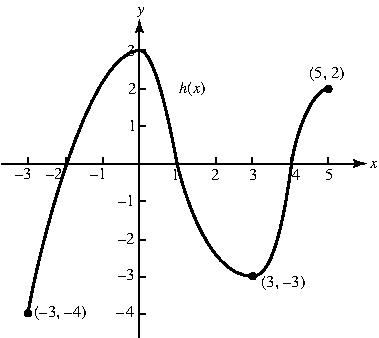
\includegraphics[width=2.5in]{images/go16p09}}
    \hspace{0.1in}
    \begin{minipage}[t]{\linewidth-2.67in}
      \vspace{0pt}
    }

  \solonly{
\includegraphics[width=2.5in]{Images/go16p09.pdf}}

  \begin{enumerate}
  \item
    \begin{problem}
      For which values of $x$ is $h'(x)$ negative?      
    \end{problem}

    \begin{solution}
      $h'(x)$ is negative whenever the graph of $h(x)$ is decreasing,
      which happens on the interval $(0, 3)$.
    \end{solution}
    
  \end{enumerate}
  \probonly{\end{minipage}}

  
  Define a new function $f(x)$ by $f(x) = [h(x)]^2$.
  \begin{enumerate}[resume]
    \item
      \begin{problem}[\vfill]
        Find all critical points of $f(x)$, and classify each as a
        local minimum, local maximum, or neither.  (\emph{Note:} This is
        asking about $f(x)$, not $h(x)$!)
      \end{problem}

    \begin{solution}
      We are looking for all $x$ such that $f'(x)$ is 0 or undefined.
      \version{Mb}{In addition, since the domain of $f$ is a closed
        interval, the endpoints $-3$ and $5$ will be critical points.}
      By the Chain Rule, $f'(x) = 2 h(x) h'(x)$.  This is never
      undefined, and it's equal to 0 when $h(x) = 0$ or $h'(x) = 0$.
      From the graph, $h(x) = 0$ when $x = -2$, $1$, or $4$, while
      $h'(x) = 0$ when $x = 0$ or $3$.  \version{1a}{So, the critical
        points of $f(x)$ are $\boxed{-2, 0, 1, 3, 4}$.}
      \version{Mb}{So, the critical points of $f(x)$ are $\boxed{-3, -2,
          0, 1, 3, 4, 5}$.}

      To classify these, let's use the First Derivative Test; that is,
      we'll make a sign chart for $f'$.  For example, let's figure out
      the sign of $f'(-2.5)$; this is equal to $2 h(-2.5) h'(-2.5)$;
      from the graph, we can see that $h(-2.5) < 0$ and $h'(-2.5) > 0$,
      so $f'(-2.5) < 0$.  The final sign chart looks like:
      \begin{center}
        \begin{tikzpicture}
          \begin{axis}[axis y line=none, x axis line style={-}, xtick={-3., -2., 0., 1., 3., 4., 5.}, xticklabels={$-3$, $-2$, $0$, $1$, $3$, $4$, $5$}, ymin=-2, ymax=2, height=1.25in, width=4in]
            \addplot+[domain=-7.:5.]{0};
            \draw (axis cs: -7., -1.5) node[right] {sign of $f'$};
            \draw (axis cs: -7., 1) node[right] {$f$};
            \draw (axis cs: -2.5, -1.5) node{$-$};
            \draw[->, xshift=2pt] (axis cs: -3, 1.5) -- (axis cs: -2.26667, 0.5);
            \draw (axis cs: -1., -1.5) node{$+$};
            \draw[->, xshift=2pt] (axis cs: -1.73333, 0.5) -- (axis cs: -0.266667, 1.5);
            \draw (axis cs: 0.5, -1.5) node{$-$};
            \draw[->, xshift=2pt] (axis cs: 0.266667, 1.5) -- (axis cs: 0.733333, 0.5);
            \draw (axis cs: 2., -1.5) node{$+$};
            \draw[->, xshift=2pt] (axis cs: 1.26667, 0.5) -- (axis cs: 2.73333, 1.5);
            \draw (axis cs: 3.5, -1.5) node{$-$};
            \draw[->, xshift=2pt] (axis cs: 3.26667, 1.5) -- (axis cs: 3.73333, 0.5);
            \draw (axis cs: 4.5, -1.5) node{$+$};
            \draw[->, xshift=2pt] (axis cs: 4.26667, 0.5) -- (axis cs: 5, 1.5);
            \draw[->, xshift=2pt] (axis cs: -2.26667, 0.5) -- (axis cs: -1.73333, 0.5);
            \draw[->, xshift=2pt] (axis cs: -0.266667, 1.5) -- (axis cs: 0.266667, 1.5);
            \draw[->, xshift=2pt] (axis cs: 0.733333, 0.5) -- (axis cs: 1.26667, 0.5);
            \draw[->, xshift=2pt] (axis cs: 2.73333, 1.5) -- (axis cs: 3.26667, 1.5);
            \draw[->, xshift=2pt] (axis cs: 3.73333, 0.5) -- (axis cs: 4.26667, 0.5);
          \end{axis}
        \end{tikzpicture}
      \end{center}
      From the sign chart, we see that $f$ has \fbox{local maxima at $x
        = 0, 3$} \\ and \fbox{local minima at $x = -2, 1, 4$}. 
    \end{solution}

    \item
    \begin{problem}[\vfill]
      Does $f$ achieve an absolute maximum on $[-3, 5]$?  If so, where?
    \end{problem}

    \begin{solution}
      Since $f$ is continuous and $[-3, 5]$ is a closed interval, $f$
      must have an absolute maximum on $[-3, 5]$ by the Extreme Value
      Theorem.  From our sign chart for $f'$, we can see that the
      absolute maximum must occur at $x = -3$, $x = 0$, $x = 3$, or $x =
      5$; to decide which one is correct, we can simply test the value
      of $f$ at all these points:
      \begin{align*}
        f(-3) &= h(-3)^2 = (-4)^2 = 16 \\
        f(0) &= h(0)^2 = 3^2 = 9 \\
        f(3) &= h(3)^2 = (-3)^2 = 9 \\
        f(5) &= h(5)^2 = 2^2 = 4
      \end{align*}
      So, $f$ has its absolute maximum at $\boxed{x = -3}$. 
    \end{solution}

  \item
    \begin{problem}[\vfill]
      Does $f$ achieve an absolute minimum on $[-3, 5]$?  If so, where?
    \end{problem}

    \begin{solution}
      Since $f$ is continuous and $[-3, 5]$ is a closed interval, $f$
      must have an absolute minimum on $[-3, 5]$ by the Extreme Value
      Theorem.  From our sign chart for $f'$, we can see that the
      absolute minimum must occur at $x = -2$, $x = 1$, or $x = 4$.
      Let's test the value of $f$ at these points:
      \begin{align*}
        f(-2) &= h(-2)^2 = 0^2 = 0 \\
        f(1) &= h(1)^2 = 0^2 = 0 \\
        f(4) &= h(4)^2 = 0^2 = 0
      \end{align*}
      So, the absolute minimum of $f$ on $[-3, 5]$ occurs at 3 points,
      $\boxed{x = -2, 1, 4}$. 
    \end{solution}

  \end{enumerate}    

\end{enumerate}

\end{document}